\documentclass[journal]{IEEEtran}                                                          % if you need a4paper
%\documentclass[a4paper, 10pt, conference]{ieeeconf}      % Use this line for a4
                                                         % paper
\IEEEoverridecommandlockouts        % This command is only
% needed if you want to
                                    % use the \thanks command
%\overrideIEEEmargins
% See the \addtolength command later in the file to balance the column lengths
% on the last page of the document
% The following packages can be found on http:\\www.ctan.org
\usepackage{graphics} % for pdf, bitmapped graphics files
\usepackage{rotating} % rotate figures
\usepackage{epsfig} % for postscript graphics files
%\usepackage{mathptmx} % assumes new font selection scheme installed
%\usepackage{times} % assumes new font selection scheme installed
\usepackage{amsmath}
\usepackage{amssymb}
\usepackage[spanish]{babel}
\usepackage{cite}

\DeclareUnicodeCharacter{0301}{\'{e}}

\usepackage{atbegshi} % erase first blank page
\usepackage{hyperref}

\AtBeginDocument{\AtBeginShipoutNext{\AtBeginShipoutDiscard}}

\title{\LARGE \bf Proyecto: Minería de datos}

%%%%%%%%%%%%%%%%%%%%%% AUTHORS %%%%%%%%%%%%%%%%%%%%%%%%%%%%%%%%%%%%%%%%5
\author{Juan Pablo Echeagaray González, Emily Rebeca Méndez Cruz, Grace Aviance Silva Arostegui}% <-this % stops 
\begin{document}

    \thanks{Juan Pablo Echeagaray González, Emily Rebeca Méndez Cruz, Grace Aviance Silva Arostegui pertencen al Tec de Monterrey campus Monterrey, N.L. C.P. 64849, Mexico {\tt\small}}

    \maketitle

    \thispagestyle{empty}
    \pagestyle{empty}

    \begin{abstract}
        Se realizó un proyecto de minería de datos en el que se probaron y documentaron 4 algoritmos de machine learning supervisados para predecir el nivel de riesgo de tener cáncer de cuello uterino. Se encontró que una red neuronal con 2 capas internas tuvo la mejor tasa de predicciones para los verdaderos positivos y el mejor puntaje F1, el inconveniente de la red neuronal fue su gran tiempo de entrenamiento.
    \end{abstract}

    \begin{IEEEkeywords} 
    Data Science, Machine Learning, SVM, Decision Tree, ANN, Logistic Regression
    \end{IEEEkeywords}

    \section{Introducción} \label{introduction}

        La base de datos fue recuperada de Kaggle (la liga de acceso se encuentra en la sección \ref{data}), para nuestro caso de estudio hemos escogido una base de datos enfocada en la clasificación de riesgo para el cáncer cervical.

        La información que contiene son  857 registros de mujeres en las que se les identifica datos, características y/o enfermedades significativas para incrementar el riesgo para contraer cáncer cervical. Entre ellos: la edad, el número de parejas sexuales, la edad de la primera relación sexual, número de embarazos, si fuma o no, el número de años fumando, el número de cajetillas consumidas por año, si consumen o no anticonceptivos, el número de años consumiendo anticonceptivos, si usan o no DIU, el número de años usando DIU, si tienen ETS o no, el número de ETS que tienen, si tienen o no los siguientes tipos de ETS (condilomatosis, condilomatosis cervical, condilomatosis vaginal, condilomatosis vulvo-perineal, sífilis, enfermedad inflamatoria pélvica, herpes, molusco contagioso, AIDs, VIH, hepatitis B, HPV, número de diagnósticos, tiempo desde el primer diagnóstico, tiempo del último diagnóstico), cáncer, CIN, HPV, Hinselmann, Schiller, citología, y biopsia.

        Las columnas de la base de datos Hinselmann, Schiller, citología, y biopsia, son variables binarias que representan diferentes estudios que tratan de encontrar cáncer en el cuello utirino de las pacientes. Dada la documentación de la base de datos, no nos fue posible determinar cuál de estos 4 estudios es el más fiable para la determinación de la presencia de un cáncer, por lo que hemos optado por la creación de una nueva variable se define como la suma de los valores que toman los estudios en la base de datos, esto resulta en una variable con 5 posibles valores, un mínimo de 0 representando un riesgo nulo o bajo de tener cáncer, y un valor máximo de 4 representando el mayor riesgo de tenerlo.

        El objetivo de nuestro proyecto es diseñar un modelo de \emph{Machine Learning} que logre predecir con alta precisión la probabilidad de que un indivuo tenga un cierto nivel de riesgo de tener cáncer.
    
    \section{Créditos} \label{credits}
       
        \begin{itemize}
            \item Juan Pablo Echeagaray González - Programador / Data Scientist
            \item Emily Rebeca Méndez Cruz - Programador / Data Scientist
            \item Grace Aviance Silva Aróstegui - Programador / Data Scientist
        \end{itemize}

    \section{Modelos de Machine Learning} \label{modelos}

        \subsection{Árbol de decisión: Emily Rebeca Méndez Cruz} \label{decision-tree}

            Los árboles de decisión son un método de aprendizaje supervisado utilizado para la clasificación y la regresión. Este método tiene como objetivo crear un modelo que prediga el valor de una variable de destino mediante el aprendizaje de reglas de decisión simples deducidas de las características de los datos proporcionados. Su estructura puede ser analizada para obtener más información acerca de la relación entre las características y el objeto a predecir \cite{agencia-b12_2021}.

            En esta representación un nodo interno representa un atributo o característica, la rama corresponde una regla de decisión y cada nodo u hoja representa el resultado. El nodo raíz es el nodo superior de un árbol de decisión.

            Al momento de crear un árbol, las observaciones de entrenamiento quedan agrupadas en los nodos terminales. Para predecir una nueva observación, se recorre el árbol en función del valor de sus predictores hasta llegar a uno de los nodos terminales \cite{rodrigo-2020}.

            La metodología de un árbol de decisión es \cite{gonzalez-2020}:
            \begin{itemize}
                \item Seleccionar el mejor atributo empleando una medida de selección de características o atributos
                \item Hacer del atributo seleccionado un nodo de decisión y dividir el conjunto de datos en subconjuntos más pequeños
                \item Comenzar la selección del árbol repitiendo el proceso en cada atributo hasta que una de estas condiciones se cumpla: \begin{itemize}
                    \item Todas las variables pertenecen al mismo valor de atributo
                    \item Se han acabado los atributos
                    \item No hay más casos
                \end{itemize}
            \end{itemize}

            Las reglas de partición ayudan a determinar puntos de ruptura para un conjunto en un nodo dado. La medida de selección de atributos es una heurística y esta proporciona un rango a cada característica, el atributo con la mejor puntuación se selecciona como atributo de división.

            Realizar el entrenamiento permite a nuestro modelo tener una base para su futura toma de decisiones, permitiendo obtener un aprendizaje inicial puesto que se le suministra información. Esto proporciona que el modelo pueda plantear correlaciones entre los datos del entrenamiento y los que tiene actualmente guiándolo a la opción correcta \cite{agencia-b12_2021}.

            \subsubsection{Implementación}

                Para la implementación se hizo uso de la clase DecisionTreeClassifier de la librería de Sciki Learn, ya que con esta función se realiza el entrenamiento del modelo. Nuestros argumentos son:
                \begin{enumerate}
                    \item X\_train(pd.DataFrame): Es el arreglo de datos con las características
                    \item y\_train(pd.Series): Arreglo con las etiquetas
                    \item max\_depth: Este da a entender la profundidad máxima del árbol, este se mantiene bajo para evitar el sobreajuste
                    \item random\_state: Controla la aleatoriedad del estimador, teniendo de valor predeterminado 0
                \end{enumerate}
                
                Se escogió una profundidad máxima de 10 después de hacer varios modelados con diferentes profundidades.
        
        \subsection{Support Vector Machine (SVM) Grace Aviance Silva Arostegui} \label{svm}
            
            Support vector machine  (SVM) es un algoritmo de aprendizaje supervisado que se utiliza en muchos problemas de clasificación y regresión, e incluso para la detección de valores atípicos \cite{geron-2019}. Este modelo de aprendizaje automático se basa en una separación de diferentes clases a través de un hiperplano en un espacio de dimensión superior \cite{deisenroth2020mathematics} \cite{mathworks-2022}.

            Dado un conjunto de muestras (ejemplos de entrenamiento) se etiquetan clases y se entrena una SVM para construir un modelo que prediga la clase de una nueva muestra.

            Para la base de datos que tenemos y el análisis que queremos llevar a cabo, en donde el enfoque es considerar en cada uno de los registros de las mujeres cual es el riesgo que tienen para desarrollar cáncer cervical. Dado que en la base de datos el rango de riesgos va de 0 a 4, tenemos así 5 clases de las cuales buscaríamos 5 hiperplanos que tengan el margen lo más ancho posible entre las clases, para así poder entregar lo mejor posible al algoritmo y hacer mejores clasificaciones futuras. Cabe mencionar que utilizamos un 80/20 de los datos para entrenamiento y prueba respectivamente.

            El objetivo de este algoritmo es encontrar un hiperplano que separe de la mejor forma posible las clases diferentes de puntos de datos, lo cual implica que el hiperplano tenga un margen lo más amplio posible entre todas las clases, paralela al hiperplano y que no tenga puntos de datos interiores o si acaso permite un número pequeño de clasificaciones erróneas.

            \subsubsection{Implementación}

                De la librería de machine learning scikit-learn para este algoritmo, importamos SVC. Definimos una función que crea y entrena un svm kernel. Creamos una variable svm la cual ejecuta la función SVM de la librería, la cual recibe tres argumentos; el tipo de kernel que en este caso fue rbf, que la clase fuese balanceada, y el random state que por default es cero.

                Entrenamos la variable con la función fit. Esta variable entrenada es indispensable ya que es la que se retorna al ejecutar el algoritmo que recibe como valores de entrada: X\_train y y\_train

        \subsection{Red Neuronal: Juan Pablo Echeagaray González} \label{neural-network}
           
            Las redes neuronales artificiales están inspiradas en las redes neuronales que encontramos en los seres vivos, la relación con estas es que decimos que estas redes artificiales están constantemente aprendiendo y modificando su conocimiento y entendimiento de un proceso, para nuestro caso de aplicación, una red neuronal artificial aprende las relaciones complejas que pueden haber entre un conjunto de variables predictoras y una variable objetivo a predecir \cite{geron-2019}.

            De forma básica, una red neuronal consiste de:
            \begin{enumerate}
                \item Capa de entrada
                \item Capas internas (o escondidas)
                \item Capa de salida
            \end{enumerate}

            \begin{figure}[!htb]
                \centering
                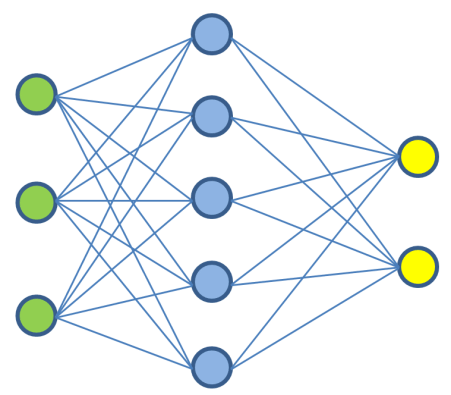
\includegraphics[scale=0.3]{../report/img/nn-diagram.png}
                \caption{Estructura básica de una red neuronal}
                \label{nn-diagram}
            \end{figure}

            Cada una de estas capas está compuesta de un número de neuronas que se conectan entre sí \ref{nn-diagram}. Si estamos hablando de un proceso de regresión o de clasificación binaria, la capa de salida solamente necesita una neurona de salida, mientras que si hablamos de un proceso de clasificación con múltiples clases, se necesitará una neurona para cada posible clase.

            Cada una de las neuronas en la red encapsulan una \emph{función de activación}, que recibe una suma ponderada de los valores arrojados por la capa anterior más un término libre. Hay diversas funciones de activación, pero las más usadas suelen ser \emph{relu} y \emph{softmax}, esta última se usa para problemas con múltiples clases \cite{geron-2019}.

            La determinación de los coeficientes usados para realizar la suma ponderada es la tarea más importante de la red neuronal, para encontrar el conjunto que optimice el desempeño del modelo se hace uso de la técnica \emph{backpropagation}, en la que en pocas palabras, la red neuronal puede darse información a sí misma de qué tan mala fue una predicción para después determinar qué coeficiente fue el que causó el mayor error.

            El número de veces que se actualizarán dichos coeficientes está primeramente en función del \emph{batch} que se le proporcione a la red. Este valor representa cuantas instancias se le pasarán a la red antes de realizar el backpropagation. Por lo general este número suele ser menor que el número de observaciones presentes en la base de datos. Una vez que la red ha hecho el número de corridas necesarias para cubrir el conjunto de entrenamiento, se dice que ha ocurrido un \emph{epoch}, esta cantidad representa el número de veces que el proceso anterior será repetido \cite{geron-2019} \cite{team-2022}.

            La naturaleza de este proceso de entrenamiento es lo que vuelve lento el proceso de entrenamiento de una red neuronal, pero también, es lo que le brinda la capacidad de ajustarse a relaciones no lineales presentes en la base de datos.

            \subsubsection{Implementación}

                Haciendo uso de la librerías \emph{Keras} y \emph{TensorFlow} hemos propuesto el siguiente diseño:
                \begin{enumerate}
                    \item Capa de entrada con 27 neuronas para los atributos que tiene la base de datos después de su limpieza. Funciónd de activación \emph{relu}
                    \item Capa de 20 neuronas. Función de activación \emph{relu}
                    \item Capa de 20 neuronas. Función de activación \emph{relu}
                    \item Capa de salida con 5 neuronas para cada uno de los posibles niveles de riesgo. Función de activación \emph{softmax}
                \end{enumerate}

                La red tiene un batch de 32 observaciones y fue entrenado por 50 epochs.

        \subsection{Regresión Logística: Juan Pablo Echeagaray González} \label{logistic}

            La regresión logística es otro de los métodos de \emph{machine learning} usados comúnmente para la clasificación de datos. Este algoritmo se usa regularmente para estimar la posibilidad de que una instancia pertenezca a cierta clase; para el caso de clasificación binaria, si dicha probabilidad es mayor al 50\%, se clasifica a esa instancia como perteneciente a la clase positiva. Para generalizar este modelo a problemas de clasificación con $n$ clases $(n > 2)$, se calculan $n$ probabilidades de que la instancia pertenezca a la clase $i$, al final se escoge la que tenga el valor más alto \cite{geron-2019} \cite{sci-kit-learn-no-dateB}.

            Al igual que con una regresión lineal, este algoritmo calcula una suma ponderada de los atributos de la instancia, más un término libre; pero lo que el modelo regresa es el resultado de aplicar la función logística a ese número:

            \begin{equation}
                \hat{p} = \sigma(\bf{x}^{T}\bf{\Theta})
            \end{equation}

            La función logística tiene un rango de 0 a 1 (por eso su uso como clasificador binario) a su vez se define como:

            \begin{equation}
                \sigma(t) = \frac{1}{1 + \exp(-t)}
            \end{equation}

            Una vez que se cuenta con la estimación de la probabilidad, la salida del modelo queda definida como:

            \begin{equation}
                \hat{y} = \begin{cases}
                    0 & \hat{p} < 0.5 \\
                    1 & \hat{p} \geq 0.5
                \end{cases}
            \end{equation}

            Para entrenar nuestro modelo hemos de encontrar el vector $\bf{\Theta} \in \mathbb{R}^{27}$ (se tienen 27 atributos después de la limpieza de datos) que minimice la función \emph{log loss}, dicha función tiene la siguiente forma:
            
            \begin{equation} \label{log-loss}
                J(\bf{\Theta}) = - \frac{1}{m} \sum_{i=1}^{m} \left[y^{(i)} \log \left(\hat{p}^{(i)}\right) + (1 - y^{(i)}) \log \left(1 - \hat{p}^{(i)} \right) \right]
            \end{equation}

            El índice $m$ de la función \ref{log-loss} representa el número de instancias que tenemos en la base de datos; lo que hace esta función es calcular el promedio del error producido con el vector $\bf{\Theta}$. Al final de la fase de entrenamiento se desea haber encontrado el vector que minimice esta función

            \subsubsection{Generalizando a n clases}

                La regresión logística que clasifica instancias que podrían tener diferentes etiquetas es conocida como \emph{Regresión Logística Múltiple} o \emph{Regresión Softmax} (similar a la función descrita en la sección \ref{neural-network}). Primero se calcula una suma ponderada como en regresión logística para cada una de las posibles clases:

                \begin{equation}
                    s_k(\bf{x}) = \bf{x}^T \Theta^{(k)}
                \end{equation}

                Se usa este valor en la función sigmoide para obtener una probabilidad estimada:

                \begin{equation}
                    \hat{p}_k = \sigma(\bf{s}(\bf{x}))_k
                \end{equation}

                Y al final se escoge la clase con la probabilidad más alta:
                \begin{equation}
                    \hat{y} = \arg\max_k \sigma(s_k(\bf{x}))
                \end{equation}
            
            \subsubsection{Implementación}

                Para nuestro caso de estudio hemos optado por utilizar la librería \emph{scikit-learn} con su regresor logístico documentado en \cite{sci-kit-learn-no-dateB}. Los datos de entrenamiento del modelo representarán un 80\% de la base de datos, y la variable que buscaremos predecir será el nivel de riesgo que tiene un individuo dados los 27 atributos que tenemos. Una comparativa de este modelo contra los demás se realizará en la sección \ref{resultados}.

    \section{Resultados} \label{resultados}
        
        Para la comparación de los modelos hemos escogido medir el \emph{recall}, el puntaje $F1$ y el tiempo de entrenamiento de los modelos. Hemos escogido estas métricas porque queremos diseñar modelos que predizcan con alta precisión los casos positivos (\emph{recall}) y queremos que en general tenga un buen desempeño de precisión y predicción de casos positivos; mientras más cercanos a 1 sean estos valores mejor; el tiempo de entrenamiento es una métrica importante a considerar también, considerar los recursos computacionales que requiere el entrenamiento de un algoritmo en especial podría definir que este sea factible o no. Para estimar el tiempo de entrenamiento de cada modelo hemos corrido una simulación en la que cada modelo fue entrenado 20 veces, al final hemos reportado el tiempo de entrenamiento promedio.
        
        Los puntajes obtenidos fueron (redondeando a 3 decimales):
        
        \begin{center}
            \begin{tabular}{ |c|c|c|c| }
                \hline
                Modelo & Recall & F1 & Tiempo (s) \\
                \hline
                Árbol de decisión & 0.793 & 0.788 & 0.024 \\
                \hline
                SVM & 0.671 & 0.659 & 0.391 \\
                \hline
                Red Neuronal & 0.826 & 0.824 & 34.836 \\
                \hline
                Regresión logística & 0.465 & 0.459 & 0.838 \\
                \hline
            \end{tabular}
        \end{center}

        Un gráfico que resume los resultados de nuestro estudio se puede ver en la figura \ref{comparison}

        \begin{figure}[!htb]
            \centering
            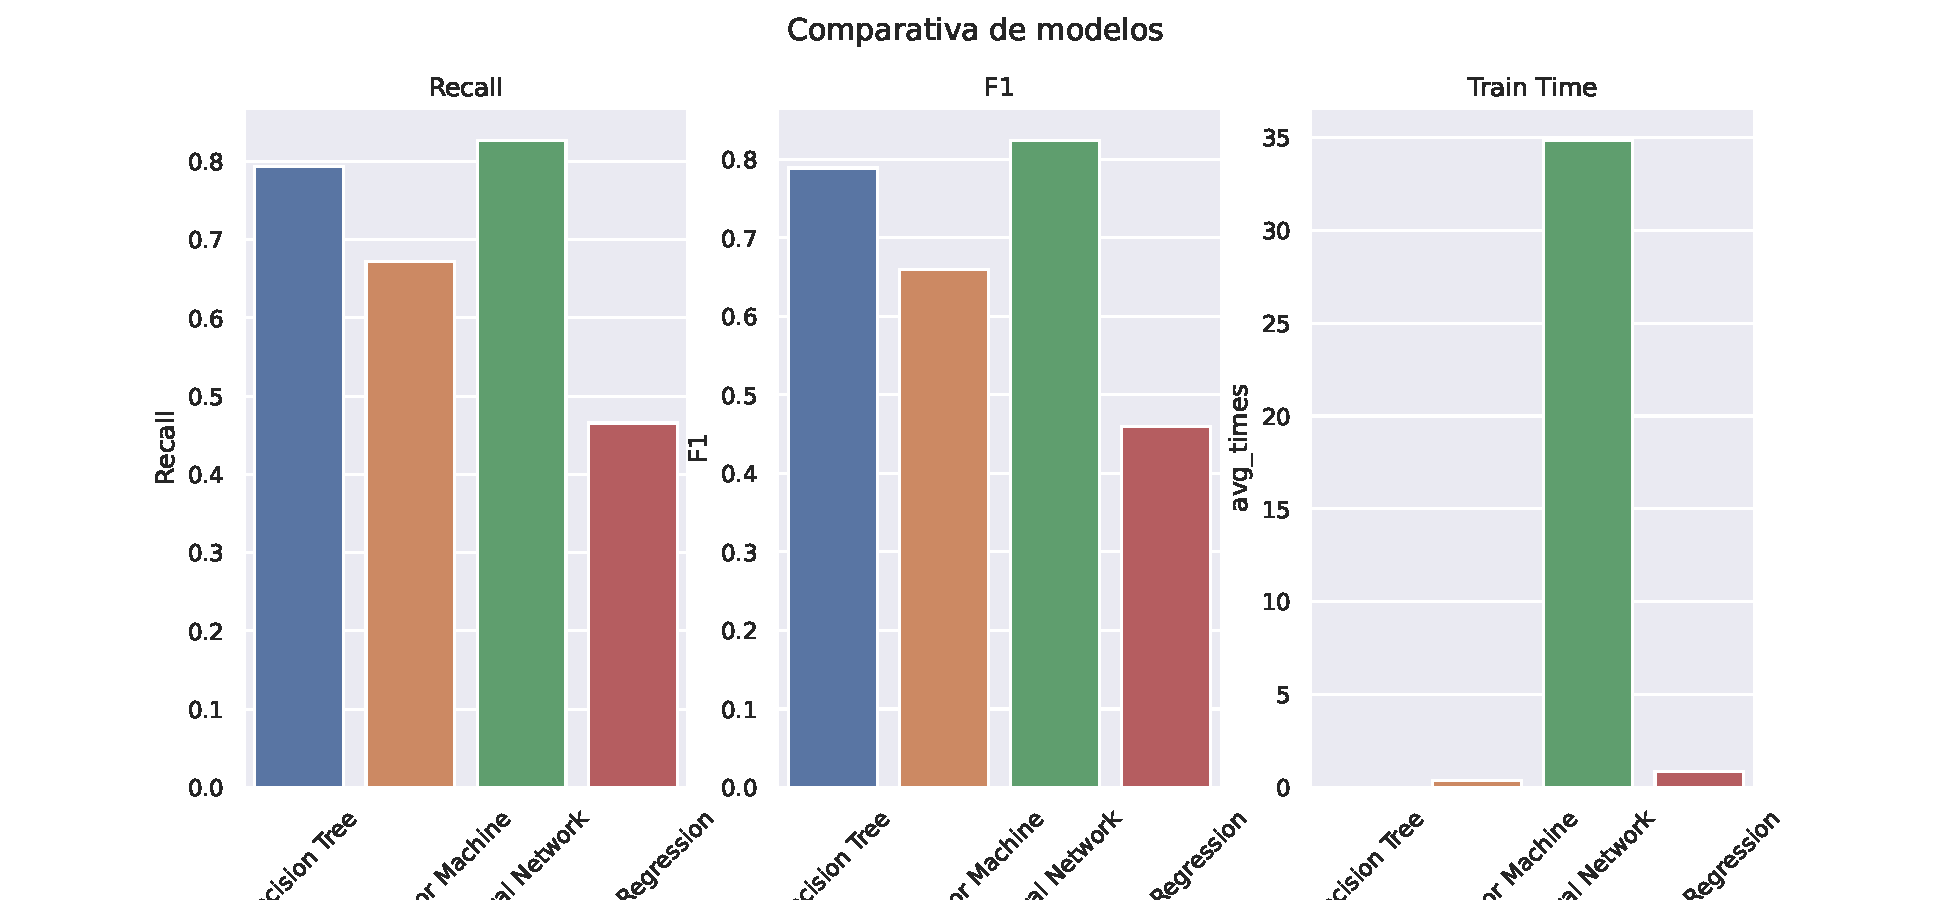
\includegraphics[scale=0.26]{../report/img/comparison-results.pdf}
            \caption{Métricas de los modelos}
            \label{comparison}
        \end{figure}

        Como vemos en \ref{comparison}, solamente el árbol de decisión, el support vector machine y la red neuronal tienen puntajes aceptables en el \emph{recall} y el puntaje $F1$. La regresión logística tuvo un desempeño mediocre, que al menos en nuestro proyecto lo remueve de la lista de posibles métodos a escoger.

        Solamente considerando estas métricas, la red neuronal tiene el mejor desempeño de los 4 modelos restantes, pero también hemos de notar que su tiempo de entrenamiento es al menos 3 ordenes de magnitud mayor.

    \section{Conclusiones} \label{conclusiones}
        
        \subsection{Áreas de mejora} \label{improvements}

            Si bien hemos encontrado modelos que tienen un desempeño aceptable para nuestro caso de estudio, el equipo reconoce que todavía hay áreas de oportunidad para mejorar el desempeño de los modelos entrenados, entre ellas se encuentran:
                
            \begin{itemize}
                \item Uso de validación cruzada para estimar el desempeño promedio de los modelos, así como encontrar los hiper-parámetros que los maximicen (donde aplique). Para el caso de la red neuronal, realizar más pruebas para encontrar la arquitectura adecuada que maximice sus puntajes.
                \item Prueba de diferentes técnicas de tratamiento de clases desbalanceadas. En nuestra aproximación se optó por usar el algoritmo KNN para la creación de datos artificiales que compensaran dicho desbalance, pero también existe la opción de añadir parámetros de regularización a los modelos usados que beneficien la predicción de las clases con un menor número de instancias
                \item Tiempo de entrenamiento de la Red Neuronal \begin{itemize}
                    \item Realizar una comparativa del tiempo de entrenamiento de la red neuronal en diferentes sistemas operativos. Al momento de la realización de nuestro estudio dispusimos de una máquina corriendo \emph{Windows 10} pero con la opción de usar una máquina virtual ligera corriendo una distribición de Linux por medio de \emph{WSL2}. El usar una distribución de Linux puede reducir drásticamente el tiempo de entrenamiento de una red neuronal dado que los drivers de las tarjetas gráficas usadas por los algoritmos que las entrenan suelen tener una mejor optimización para estos sistemas operativos.
                    \item Aunado a esto, existe la posibilidad de usar tarjetas gráficas para acelerar este proceso aún más, por motivos de recursos, esta área de oportunidad quedaría completamente fuera de nuestro alcance, pero está demostrado que el uso de estas tarjetas mejora el tiempo de entrenamiento de las redes neuronales \cite{likhith-k-2019}.
                \end{itemize}
            \end{itemize}
            
        \subsection{Modelo seleccionado} \label{selected-model}
            
            El modelo que hemos seleccionado es la Red Neuronal, tuvo el mayor puntaje de \emph{Recall} y del puntaje $F1$. Creemos que el tiempo de entrenamiento del modelo podría ser drásticament reducido como lo hemos discutido en la sección \ref{improvements}. El coste de un tiempo extra de implementación así como una inversión monetaria en un equipo computacional con mayor poder se vuelven restricciones triviales cuando se trata de diagnosticar la presencia de cáncer en una persona.

    \section{Reflexiones} \label{thoughts}

        \subsection{Juan Pablo Echeagaray González}
            
            El trabajar con datos médicos será siempre una tarea complicada desde el ámbito ético. Desde la perspectiva de que se debe de respetar la privacidad de los individuos hasta el diseño de diferentes modelos predictivos que no se encuentren sesgados hacia un grupo poblacional en específico. Creo que el deber de un buen científico de datos es siempre garantizar que el uso de los datos que tenga disponibles no comprometan en ninguna manera la privacidad de las personas que se encuentren en la base de datos.

            En caso de que el investigador disponga de alguna manera de identificar a los individuos de forma general, también será su deber el evitar que su algoritmo se sesgue para generar resultados favorables para cierto sector de la población.

            Este proyecto reresentó un gran salto en mi aprendizaje de la Ciencia de Datos y el Machine Learning, al menos hasta este punto nunca había implementado ni estudiado tan a fondo una red neuronal; todavía me falta mucho por recorrer para generar modelos más eficaces, pero me alegra haber comenzado esta etapa de aprendizaje.

        \subsection{Emily Rebeca Méndez Cruz}

            Gracias a esta actividad puedo darme cuenta de cuán importante es tener una buena base de datos para la predicción de alguna enfermedad, ya que se debe de dar la predicción con la mayor precisión posible para este tipo de situaciones. Debido a que estamos trabajando con personas, tenemos la vida de personas en nuestras manos, por lo que es una gran responsabilidad para la gente que trabaja en esta área.

            El uso de la tecnología en la medicina ha abierto una gran panorama de posibilidades tanto para el tratamiento de un paciente o para la predicción de un posible caso. El uso de estos modelos nos permiten identificar pacientes de alto riesgo de alguna enfermedad, permitiendo identificar y anticiparse a las necesidades de los pacientes. También se puede predecir la evolución de los pacientes debido a que con esta información se pueden tomar las medidas necesarias para evitar una propagación de la enfermedad.

            Este proyecto es una nueva forma de ver el análisis de datos, ya que me permitió visualizar una nueva forma de hacer uso de este y cómo se puede emplear para ayudar a otros e inclusive salvar sus vidas. Me permitió también aprender más acerca de lo que estoy estudiando a lo largo de esta etapa de mi vida.
        
        \subsection{Grace Aviance Silva Arostegui}

            Sin duda, el desarrollo de la medicina junto con la tecnología es una gran apuesta para un acercamiento a una mejor calidad de vida e incluso para la aspirada sociedad 5.0 cuya característica principal es que los avances tecnológicos contribuyan significativamente a una mejora de la sociedad en al que se enfoca todo su esfuerzo en beneficiar al ser humano. Reflexiono la importancia de las implicaciones profesionales que conlleva el desarrollo y análisis médicos por parte de profesionistas que no son médicos; en toda profesión hay responsabilidad en las manos de los proyectos que se llevan a cabo, más el trabajar con datos médicos es un tema muy delicado ya que la salud es lo más importante y frágil para las personas. Estas implicaciones profesionales van desde lo que es el llenado de estas bases de datos, porque de no ser bien registradas o medidas meticulosamente, pueden afectar los análisis, resultados, recomendaciones y predicciones para los pacientes y así dar malos pronósticos o recetas médicas, e inclusive afirmar que ciertos pacientes no tengan probabilidad o se encuentren en riesgo de desarrollar alguna enfermedad dando un falso negativo, y esto refleja directamente el tema ético y de negligencias médicas. Es de suma importancia que todo el proceso sea muy minucioso y ordenado para poder sacar el mejor provecho del desarrollo de la tecnología y sus áreas multidisciplinares que se relacionen con las aplicaciones médicas.

            Me agradó este proyecto ya que fue un buen primer acercamiento de aplicación médica a Data Science, el poder comparar distintos algoritmos de machine learning para poder clasificar registros y predicciones de riesgo para desarrollar cáncer. Me parece de gran valor el poder darle uso al área médica los conocimientos de mi carrera, y el hecho de que pueden tener un impacto positivo en la sociedad.
        
    \appendices
    
    \section{Datos} \label{data}
        
        Base de datos consistente de 36 características y de 858 observaciones. Está compuesta principalmente de variables categóricas que indican si alguna enfermedad o afección se encontró presente en el individuo. Consta de pocas variables numéricas como lo son la edad, el número de embarazos y de parejas sexuales, la edad en la que se tuvo la primera relación sexual y el número de años que ha fumado.
            
        Los datos usados en este proyecto pueden descargarse \href{https://www.kaggle.com/code/ravaliraj/risk-classification-of-cervical-cancer}{aquí}.

    \section{Código}\label{repo}

        El código desarrollado se encuentra en el siguiente \href{https://github.com/JuanEcheagaray75/cancer-clf}{repositorio}.
    \section{Evidencias de trabajo en equipo}
        
        En este \href{https://docs.google.com/document/d/1febGMKH0Z8mdPzhVf\_FTBrOR3ENYA2iGw5Lfeg8XTjk/edit?usp=sharing}{link} se puede ver un historial del borrador usado para generar este reporte, ahí se pueden ver las contribuciones hechas por cada integrante al producto final. Las aportaciones de Juan Pablo Echeagaray González pueden ser vistas desde el historial de commits en el repositorio proporcionado en la sección \ref{repo}.

    \bibliographystyle{IEEEtran}
    \bibliography{references.bib}

\end{document}